%%%%%%%%%%%%%%%%%%%%%%%%%%%%%%%%%%%%%%%%%%%%%%%%%%%%%%%%%%%%%%%%%%%%%%%%%%%%%
\chapter{Verwandte Arbeiten}
\label{chap:related}
%%%%%%%%%%%%%%%%%%%%%%%%%%%%%%%%%%%%%%%%%%%%%%%%%%%%%%%%%%%%%%%%%%%%%%%%%%%%%
\chapterstart
Das Kapitel „Verwandte Arbeiten“ dient dazu, einen umfassenden Überblick über bestehende Forschungen und Entwicklungen im Bereich der Web-Crawler Technologien zu geben. Dieses Kapitel strukturiert und gruppiert relevante Studien und Ansätze systematisch, um die Vielfalt der Forschungslandschaft aufzuzeigen und die eigene Arbeit klar innerhalb dieses Spektrums zu positionieren. Durch die Analyse und Diskussion verwandter Arbeiten wird nicht nur der Stand der Technik dargelegt, sondern auch der Beitrag der eigenen Forschung hervorgehoben.

\section{Cloud-basierte Services im Web-Crawling}

Im Rahmen der fortschreitenden Entwicklung von Web-Crawler Technologien stellt der Ansatz des Artikels mit dem Titel \textit{\citetitle{ElAraby2018}~\parencite[vgl.][]{ElAraby2018}} eine Basis für die Skalierung von Web-Crawlern dar. Dieser Ansatz hebt die Bedeutung einer serviceorientierten Architektur hervor, die auf Cloud-Computing basiert, um die Skalierbarkeit von Crawlern zu verbessern. Ein besonders bemerkenswerter Aspekt ist die Intention der Autoren, einen sogenannten ''Crawling-Service'' zu entwerfen, der sich durch seine unabhängige Skalierbarkeit auszeichnet. Die Abbildung \ref{fig:CrawlerServiceElAraby1} visualisiert die Zielarchitektur des Werkes.

%Besonders hervorzuheben ist die Absicht der Autoren einen sogenannten ''Crawling-Service'' %konzipierten, welcher unabhängig skalierbar ist. 
\begin{figure}[H]
    \centering
    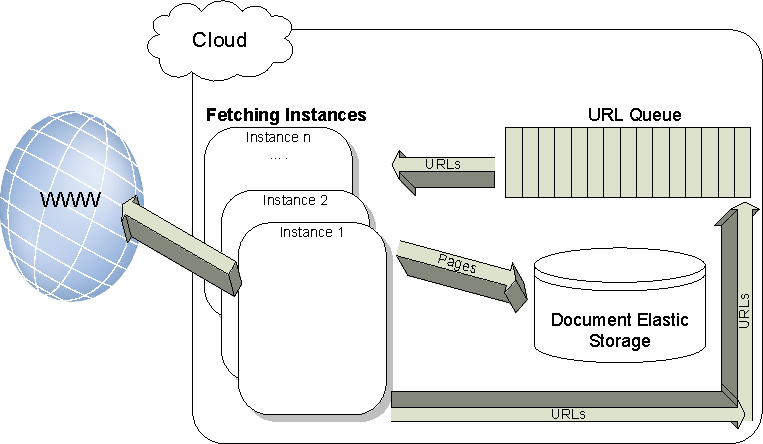
\includegraphics[width=13cm]{images/20_related/group-MC15.pdf}
    \caption[Visualisierung von Crawling Instanzen]{Visualisierung der sogenannten Crawling Instanzen innerhalb der Zielarchitektur~\parencite[vgl.][S. 4]{ElAraby2018}.}
    \label{fig:CrawlerServiceElAraby1}
\end{figure}
Der Service stellt eine Web-Crawling Lösung dar, die in Form einer einzelnen Applikation realisiert ist. Trotz der Möglichkeit zur unabhängigen Skalierung, weist die Instanz eine monolithische Architektur auf. Zusätzlich kommt ein alternativer Ansatz zur Skalierung zum Einsatz, der die Existenz mehrerer, unabhängig voneinander funktionierender URL-Queues vorsieht, wie in Abbildung \ref{fig:CrawlerServiceElArabyGlobal} dargestellt.

\begin{figure}[H]
    \centering
    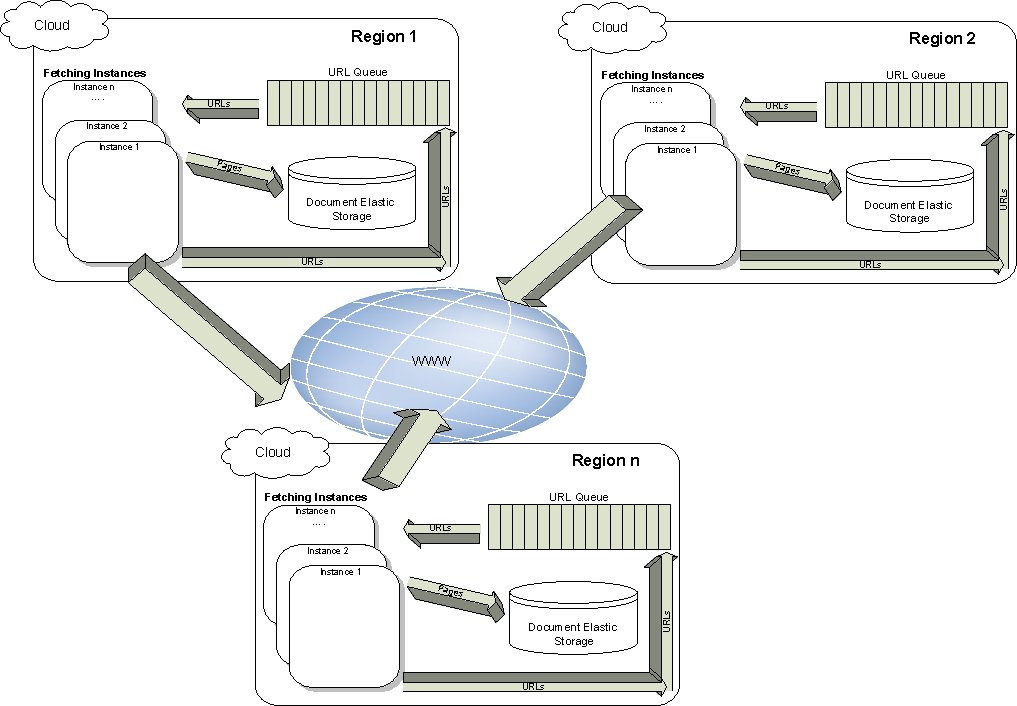
\includegraphics[width=13cm]{images/20_related/group-MC17.pdf}
    \caption[Visualisierung geographisch verteilter Crawler]{Visualisierung geographisch verteilter Crawler der Zielarchitektur~\parencite[vgl.][S. 4]{ElAraby2018}.}
    \label{fig:CrawlerServiceElArabyGlobal}
\end{figure}

Im Gegensatz zur zuvor erwähnten Arbeit mit dem Titel \textit{\citetitle{ElAraby2018}~\parencite[vgl.][]{ElAraby2018}{}{}} repräsentiert diese Arbeit eine Weiterentwicklung und konkretisiert die nächste Stufe dieser konzeptionellen Grundlage. Sie geht über die \ac{SOA} Architektur hinaus, indem sie eine noch feingliedrigere Unterteilung in unabhängige Services vornimmt. Um die aufgestellte Hypothese zu erfüllen, wird in diesem Sinne eine Microservice-basierte Architektur entwickelt.

Im Vergleich zu einer serviceorientierten Architektur, welche detailliert in Abschnitt \ref{subsec:monoservmicro} im Kontrast zu Microservices diskutiert wird, bietet letzterer Ansatz eine verbesserte Präzision und Effizienz in der Steuerung der Services. Diese Vorteile gehen jedoch mit einer gesteigerten Komplexität einher. In Abschnitt \ref{subsec:monoservmicro} werden die Vor- als auch Nachteile von Microservices nochmals umfassend beleuchtet.

In der Architektur dieser Arbeit werden nicht einzelne, gleiche Service-Instanzen eingesetzt, sondern es findet eine Synergie mehrerer, verschiedener Services statt. Darüber hinaus werden diese Microservices in einer Cloud-nativen Umgebung eingebettet. Durch die Cloud-nativen Ansätze kann nochmals eine Optimierung der Skalierbarkeit erreicht werden. Dies wird in Kapitel \ref{sec:cloudnative} beschrieben.
\section{Optimierung der Performance mit \acl{AOT}}
Im Kontext der zunehmenden Komplexität moderner Softwareentwicklung und der Notwendigkeit, diverse Technologien sowie verschiedene Programmiersprachen zu integrieren, beleuchtet der Artikel unter dem Titel \citetitle{8756917}~\parencite[vgl.][]{8756917} die Rolle der GraalVM als innovativen Ansatz. Diese Forschungsarbeit unterstreicht die Bedeutung der GraalVM für die Verbesserung der Interoperabilität zwischen Programmiersprachen bei gleichzeitiger Optimierung der Leistung. 

Der zentrale Fokus liegt auf dem in Java entwickelten Graal-Compiler, der sowohl als \ac{JIT}- als auch als \ac{AOT}-Compiler fungiert und durch seine fortgeschrittenen Optimierungstechniken, insbesondere im Hinblick auf Algorithmen, die Entwicklung und Wartung von Software beschleunigt und vereinfacht. 
\newpage
Die Arbeit hebt hervor, wie die GraalVM durch ihre Architektur und Funktionalitäten das Software-Ökosystem bereichert, indem sie eine nahtlose Integration und effiziente Ausführung von Anwendungen in verschiedenen Programmiersprachen wie Java, JavaScript, C/C++, Python, Ruby und R ermöglicht.

Das genannte Werk beleuchtet die Unterschiede zwischen \ac{AOT} und \ac{JIT} Kompilierung über verschiedene Programmiersprachen hinweg, mit einem besonderen Fokus auf die Optimierung von \ac{JVM}-basierten Sprachen. Diese Arbeit jedoch erweitert die Untersuchung, indem sie die Effektivität der Optimierung in einem praxisnahen Einsatzszenario evaluiert. Wie in \citetitle{8756917}~\parencite[vgl.][]{8756917} erwähnt, basieren die vorläufigen Testergebnisse auf einem begrenzten Umfeld, woraus der Plan entstand, die Forschung durch Experimente in einem umfangreicheren Kontext fortzusetzen.

Entsprechend knüpft die vorliegende Arbeit an dieser Stelle an, indem sie die Wirksamkeit der AOT-Optimierung in einer realitätsnahen, cloud-nativen Umgebung untersucht, in der die Anwendungen integriert sind. Die Untersuchung erstreckt sich dabei auf einen Bereich, in dem bisher wenig Forschung vorliegt: den spezifischen Anwendungskontext von Web-Crawling.

Diese Arbeit zielt darauf ab, diese Lücke zu schließen, indem sie die Anwendbarkeit und Vorteile der \ac{AOT}-Optimierung für Web-Crawling in einer Cloud-nativen Umgebung untersucht. Die Analyse konzentriert sich auf die Herausforderungen und Anforderungen, die für das Web-Crawling spezifisch sind. 

\vfill

\chapterend